\section{Bonus Features}
\label{sec:bonus}

The assignment proposes several bonus improvements: machine learning, event correlation, geolocation, and adaptive scoring. RAPID implements or demonstrates all of them in a way that extends the main Lambda Architecture.

\subsection{Machine Learning Classification}

The \texttt{ml\_bonus.py} script trains a Spark MLlib Random Forest classifier to predict \texttt{threat\_label} from features such as transferred bytes, protocol, action, and log type. The objective is not to replace rule-based detection, but to show that the same Big Data pipeline can support statistical classification. The model reached about 92\% global accuracy, while the report also recognizes that class imbalance can hide errors on minority malicious classes.

\begin{figure}[H]
    \centering
    
\includegraphics[width=0.92\textwidth]{\detokenize{figures/bonus_features/Screenshot 2026-05-07 172733.png}}
    \caption{Spark MLlib model evaluation and saved prediction output.}
    \label{fig:ml-results}
\end{figure}

\subsection{Multi-Step Attack Correlation}

The batch layer includes a multi-step detector that correlates different attack families for the same source IP. For example, a source that performs tool scanning, SQL injection, and path traversal is more dangerous than a source with one isolated event. This bonus improves the quality of historical prioritization.

\begin{figure}[H]
    \centering
    
\includegraphics[width=0.90\textwidth]{\detokenize{figures/bonus_features/3.png}}
    \caption{Enriched multi-step attack correlation with risk level.}
    \label{fig:multistep}
\end{figure}

\subsection{Adaptive Threshold and Geolocation-Oriented View}

The API includes an adaptive threshold calculation based on recent activity. Instead of relying only on a fixed score, the system compares an IP against the current context of the platform. The dashboard also includes a global map view for attack visualization, which supports the geolocation improvement proposed in the assignment.

\begin{figure}[H]
    \centering
    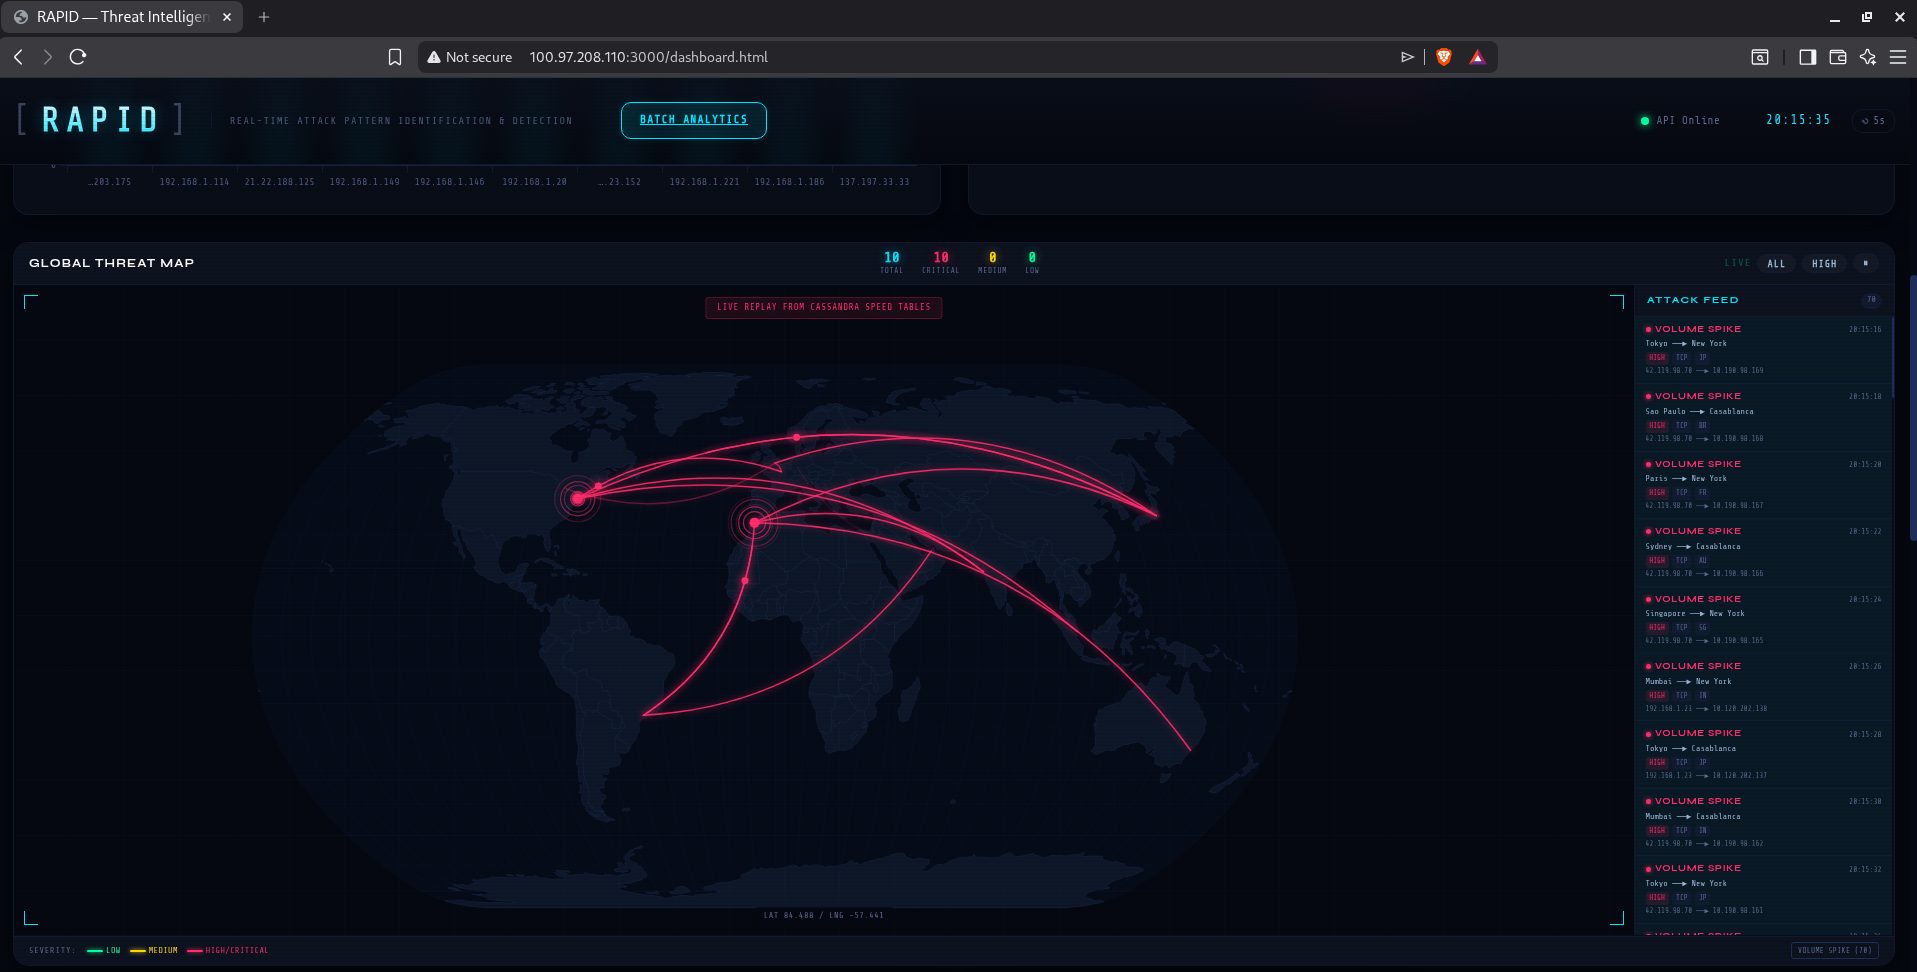
\includegraphics[width=0.92\textwidth]{figures/serving/speed_dashboard/speed_dashboard_global_threat_map.png}
    \caption{Global threat map used to visualize attack origins and trajectories.}
    \label{fig:global-map}
\end{figure}

These bonuses show that RAPID is extensible. New detectors can be added as Spark jobs, new serving views can be materialized in HBase or Cassandra, and the API can expose new indicators without changing the core architecture.
